% !TeX encoding = ISO-8859-1
% !TeX spellcheck = fr_FR

\newpage
\section{Position du joueur}

\subsection{Les pieds} 
Les pieds doivent �tre stables, l�g�rement �cart�s de mani�re � assurer une surface au sol la plus large possible (\autoref{fig:a01-a}).
Une bonne assise permet un bon �quilibre sans d�pense d'�nergie inutile et un bon positionnement face au jeu.

\subsection{ Les jambes} 
�galement �l�ments de stabilit�, elles doivent supporter le poids du corps uniform�ment. 
Jamais, une jambe seule ne doit supporter le poids du corps, sauf s'il est impossible de poser les deux pieds au sol ! Si on doit forcer sur une jambe pour garder l'�quilibre, cela peut �tre une source d'impr�cision voire d'erreur de jugement. Les jambes doivent �tre l�g�rement fl�chies, comme si on �tait pr�t � s'asseoir sur une chaise. 
Cette position permet une orientation correcte du tronc. 
Au d�but, elle semblera un peu p�nible. 
Avec le temps, il sera possible d'am�nager des corrections de confort sans alt�rer le jugement du joueur : avancer un
pied, s'aplatir le tronc sur la canne ou raidir une jambe. \'A chacun de voir, mais retenons qu'une assise souple est toujours pr�f�rable � une assise raide.

\subsection{Le tronc} Le tronc est face � la direction choisie,
fermement stabilis�, inclin� vers l'avant. Id�alement,
le menton, le nombril et la bille 1 devraient �tre parfaitement align�s.
Seul un contorsionniste pourrait y arriver mais il faut tenter de
s'en rapprocher. Dans ses conditions id�ales, la vue du
joueur est situ�e � la verticale de cette droite (\autoref{fig:a01-b}).

\begin{figure}
	\centering
	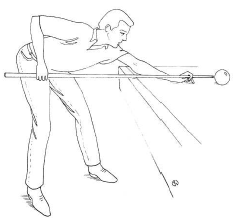
\includegraphics[width=0.7\linewidth]{A/imagesA/A01-a}
	\caption{Position du corps.}
	\label{fig:a01-a}
\end{figure}
\begin{figure}
	\centering
	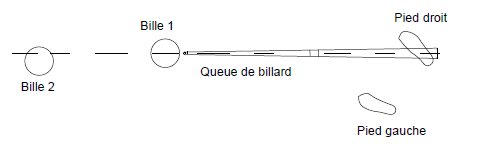
\includegraphics[width=0.7\linewidth]{A/imagesA/A01-b}
	\caption{Vue du dessus.}
	\label{fig:a01-b}
\end{figure}



